\documentclass[../../main]{subfiles}

\renewcommand\thesection{\arabic{section}}


\begin{document}

\section{Exhaust Branches and Inlet} \label{sec:exhaustBranchesAndInlet}

The core block alone cannot properly manage the thermals of the incubator.
Along with that, we need some way to replenish the air inside the incubator.
Exhaust branches and inlet ports does exactly that.

\begin{center}

    \begin{tabularx} {\textwidth} {
            >{\centering \arraybackslash}X
            >{\centering \arraybackslash}X
        }

        \toprule

        Exhaust Branches & Exhaust Inlets \\

        \midrule

        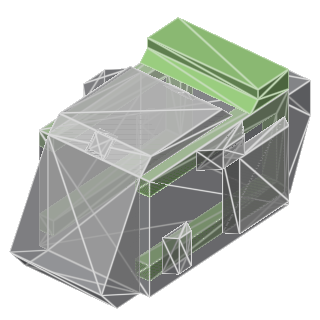
\includegraphics [
            height = 0.18\textheight,
        ] {pics/ext_right.png}

        &

        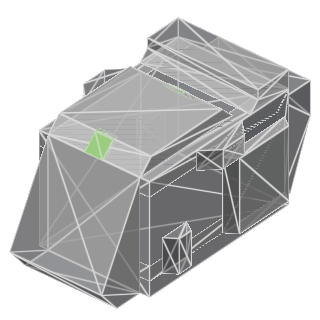
\includegraphics [
            height = 0.18\textheight,
        ] {pics/ext_inlets_right.png}

        \\
        \vspace{-0.5cm}

        \captionof{figure}[Exhaust branches with core block.]{}
        \label{fig:exhaustBranches}

        &

        \vspace{-0.5cm}
        \captionof{figure}[Exhaust inlet ports.]{}
        \label{fig:exhaustInlets}

        \\

        \bottomrule

    \end{tabularx}

\end{center}

\alertImportant{
    Look closer at figure \ref{fig:exhaustBranches}, both the ports of each bottom panel are connected
    together and branches to either sides of the incubator.
}

% \alertWarning{
%     The exhaust pipes in figure \ref{fig:}
%     The final implementation of the exhaust branches will differ from
% }

Each branch will have two fans associated with them. These four fans are directed away
from the center of the incubator. The two exhaust inlets are covered using two panels,
and there will be a fan associated with each of them. These two fans are directed towards
the center of the incubator. Depending on the mode of the core block, these three pairs of
fans are activated or deactivated. Refer table \ref{tbl:differentFanStates} to know
the states of these three pairs of fans, given that the core block in one of its active modes.

\begin{center}

    \begin{tabularx} {\textwidth} {
            >{\ttfamily \centering \arraybackslash}m{2cm}
            >{\ttfamily \centering \arraybackslash}X
            >{\ttfamily \centering \arraybackslash}X
            >{\ttfamily \centering \arraybackslash}X
        }

        \toprule

        MODE & RIGHT SIDE FANS & LEFT SIDE FANS & INLET FANS \\

        \midrule

        CMODE & INACTIVE & ACTIVE & INACTIVE \\
        HMODE & ACTIVE & INACTIVE & INACTIVE \\
        EMODE & ACTIVE & ACTIVE & ACTIVE \\

        \bottomrule

    \end{tabularx}

    \captionof{table} {Different core block modes and corresponding state of different fans.}
    \label{tbl:differentFanStates}

\end{center}

\end{document}
